\section{Experiments}\label{s:exp}
Next, we present experimental results that suggest two main conclusions: (1) as a single framework, \sys achieves parity in terms of accuracy with state-of-the-art approaches to a variety of different problems ranging from integrity constraint satisfaction, statistical data cleaning, and also data cleaning for machine learning, (2) while the serial implementation of \sys can be much slower than the competitor specialized frameworks, \sys can be efficiently distributed to significantly reduce the gap.

\begin{figure}
    \centering
    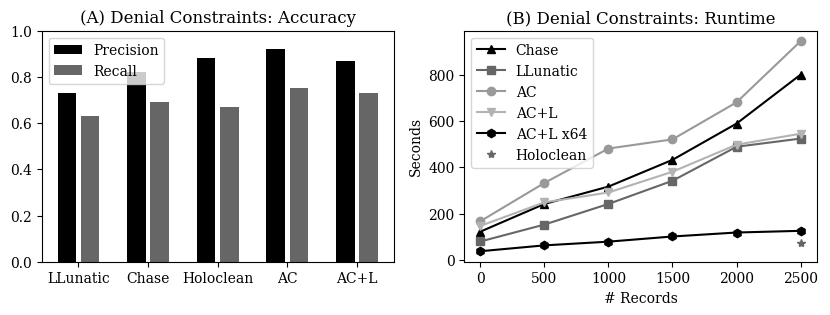
\includegraphics[width=\columnwidth]{exp/exp1.png}
    \caption{We compare \sys to alternative denial constraint systems on a dataset of flight arrival and departure times scraped from a variety of different sources. AC denotes \sys without any learned pruning and AC+L denotes \sys with pruning.
    \sys matches the accuracy of these systems and can be parallelized to match the runtime of these systems as well. Learning actually allows \sys to scale sub-linearly, i.e., as it sees more data it learns more precise pruning rules.\label{exp1a}}
\end{figure}

\subsection{Comparisons}
First, we compare \sys to a number of different baselines. To set expectations, \sys is a more general framework and we illustrate that it can match the accuracy of many more specialized frameworks. It is however slower in terms of runtime on certain problems. The goal of this section is to illustrate this tradeoff.

\subsubsection{Denial Constraints}
Denial Constraints are a logical language for specifying integrity constraints with universal quantification (e.g., all employees must earn less than his or her manager).
Several data cleaning systems use Denial Constraints for constraint specification. 
While \sys does not enforce integrity constraints, we can create a data quality objective function that quantifies the number of unsatisfied constraints.
This will search over a set of transformations that maximally satisfy these constraints.

\vspace{0.5em}\noindent\textbf{Flight Dataset: } The flight dataset contains arrival time, departure time, and gate information aggregated from 3 airline websites (AA, UA, Continental),
8 airport websites (such as SFO, DEN), and 27 third-party
websites.
There are 1200 flights departing from or arriving at the hub airports of the three airlines) from each source.
The data cleaning problem is to reconcile the differences between each sources.
Each flight has a unique flight identifier that is consistent across the websites.
Formally, we can model the reconciliation problem as functional dependency between the flight id and the arrival time, departure time, gate information.
This enforces that after resolution there will be a single canonical version of those values.

\vspace{0.5em}\noindent\textbf{Baselines: } We compare to two baselines: (1) Llunatic a denial constraint-based data cleaning systems~\cite{DBLP:conf/sigmod/DallachiesaEEEIOT13}, which is a C++ system implemented on Postgres SQL and (2) a restricted chase algorithm as in ~\cite{benedikt2017benchmarking} implemented in Python. We also present numbers for comparison from a recently published system called Holoclean~\cite{rekatsinas2017holoclean} on the same datasets, but did not run the experiment ourselves.


\vspace{0.5em}\noindent\textbf{Results: } Figure \ref{exp1a} plots the results of this experiment. Figure \ref{exp1a}a shows the precision and recall of the various approaches w.r.t a gold-standard ground truth. \sys matches the accuracy of the other denial constraint based systems. Figure \ref{exp1a}b illustrates the runtime. While \sys without any learning is quite slow compared to the alternatives, learning can speed up the cleaning process significantly.
In fact, the results suggest that the scaling is \emph{sublinear}, where as the system sees more data it becomes more effective at pruning bad search branches.
For reference, we additionally include results parallelizing \sys on a 64 core machine with 64 search threads. This roughly matches the performance reported by Holoclean. 


\vspace{0.5em}\noindent\textbf{Other Datasets: } We also evaluated \sys on three  other datasets:
\begin{enumerate}
    \item The FEC provides a dataset of election contributions of 6,410,678 records with 18 numerical, categorical and string valued attributes. This dataset records the contribution with various demographic information about the contributors including name, address, and occuption.
    In this dataset, we enforced functional dependency relationships between city and zipcodes. We also matched the occupation of the contributors to a code book of popular occupations. This was posed as a quality function that was 1 only if the cell belonged to the code book and 0 otherwise, and there was an additive penalty on the edit distance between the change and the previous value.   
    \item The Malasakit dataset contains survey responses on disaster preparedness from the Philippines with 15 numerical and categorical attributes. In this dataset, we removed numerical outliers and pruned test data from the dataset. 
    \item The Physican dataset from  Medicare.gov contains information on physicians from the United States. There are a number of inconsistencies such as  spelling errors in the city names, zip code formatting, other organization name inconsistencies.
\end{enumerate}

The results are presented below with precision, recall, and a single-threaded runtime.
\begin{table}[ht]
\footnotesize
\centering
\begin{tabular}{|l|r|r|r|r|r|r|r|}
\hline
 & \#rows & \#cols & Pre & Rec & Runtime (s) \\
\hline
\hline
FEC	&6410678&18&0.94&	0.68&	18270s\\
\hline
Malasakit &1493& 15& 1.0 & 0.85& 1404s\\
\hline
Physican	&37465&10&1.0&0.84& 11761s\\
\hline
\end{tabular}
\end{table}

\begin{figure}
    \centering
    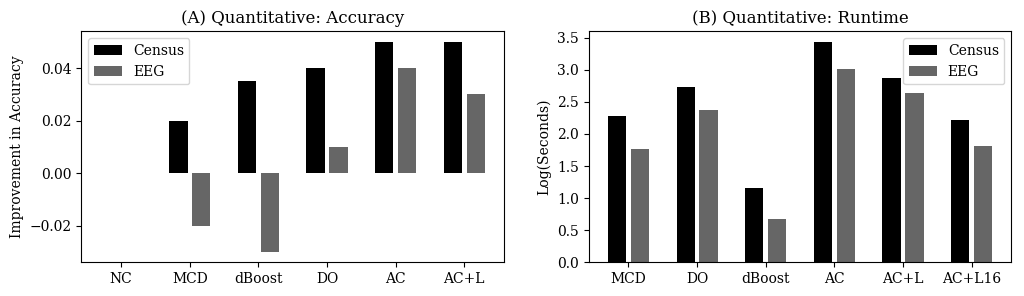
\includegraphics[width=\columnwidth]{exp/exp2.png}
    \caption{We evaluate \sys on a quantitative data cleaning task by cleaning a dataset prior to training a random forest classifier model. NC denotes no cleaning, MCD denotes using a Minimum Covariance Determinant approach to remove statistical outliers, DO denotes \label{exp1a}}
\end{figure}

\subsubsection{Quantitative Data Cleaning}
In this experiment, we consider handling numerical outliers in ML datasets.
In many machine learning settings, cleanly labeled test data is often available (e.g., the results of following a sales lead). 
Labels often represent directly observed phenomena making them relatively clean, while features are often weaker signals integrated from multiple disparate sources and subject to error and frequent change.
This allows us to define a quality function in terms of the model's predictive accuracy--the data cleaning being a means to improving that predictive accuracy.

\vspace{0.5em}\noindent\textbf{USCensus: } This dataset contains US Census records for adults and the goal is to predict  whether the adult earns more than $50,000$ dollars. It contains 32,561 records with 15 numerical and categorical attributes. This dataset contained a significant number of missing values coded as 999999.

\vspace{0.5em}\noindent\textbf{EEG: } This is a dataset of EEG recordings. 
The training data is organized into ten minute EEG clips labeled "Preictal" for pre-seizure data segments, or "Interictal" for non-seizure data segments. 
There are 2406 records each of which is a variable-length time-series of 16 attributes. We featurize this dataset into records of 32 attributes--the mean and variance over the length of the time-series. 
This dataset primarily contains numerical outliers, the clips have spurious readings.

\vspace{0.5em}
We defined a prediction task on each of these datasets. We trained a \textsf{sklearn} Random Forest classifier to predict the labels. The training procedure uses a set of standard featurizers (hot-one encoding for categorical data, bag-of-words for string data, numerical data as is) in a similar fashion as~\cite{gokhale2014corleone}. The quality function for \sys is 0 for each record that is incorrectly predicted by the model, 1 for each record that is correctly predicted by the model.

\sys is allowed to search through modifications to the records to try to make the prediction correct. We focused on transformations to numerical columns. Allowed data transformations are:
\[
\textsf{clip\_above}(attr, threshold), 
\]
which sets all values in $R[attr]$ above the threshold to threshold.
\[
\textsf{clip\_below}(attr, threshold), 
\]
which sets all values below threshold to threshold.
\[
\textsf{set\_default}(attr, value), 
\]
which sets all values in $R[attr]$ equal to value to the mean value.


\subsubsection{Baselines}

\vspace{0.5em}\noindent\textbf{Baselines: } For this experiment, we defined a 20\% held-out test dataset. We apply the search on the 80\% of the training data, and apply the discovered transformations before predictions on the 20\% held-out set. 
We compare to the following baselines: (No Cleaning) there is no modification to the data before prediction, (Minimum Covariance Determinant) we apply a standard outlier detection technique that does not consider the subsequent trained model and sets all detected outliers to the mean value, and (Default Only) we run \sys where the only operation is setting the mean value.



\begin{table}[ht]
\footnotesize
\centering
\begin{tabular}{|l|r|r|r|r|r|r|r|}
\hline
Pred. Accuracy & \#rows & \#cols & NC & MCD & DO & AC \\
\hline
US Census	&32561&15&0.82&	0.79&	0.86&	\pop{0.87}\\
\hline
EEG	&2406&32&0.79&	0.81&	0.80&	\pop{0.83}\\
\hline
\end{tabular}
\end{table}

\textbf{Sk. TODO it's slow but it works}
\begin{table}[ht]
\footnotesize
\centering
\begin{tabular}{|l|r|r|r|r|r|r|r|}
\hline
Runtime (s) & \#rows & \#cols & NC & MCD & DO & AC \\
\hline
US Census	&32561&15&-&\pop{187.12}&545.96&731.59\\
\hline
EEG	&2406&32&-&\pop{57.52}&236.11&437.10\\
\hline
\end{tabular}
\end{table}


\ewu{Other than the fact that AC is good, did we learn anything else?  Do we want to vary the number of columns in the datasets?  }

















\vspace{0.5em}\noindent\textbf{FEC Dataset: }  We can calculate the semantic similarity between two occupations with a \textsf{word2vec} model.

\vspace{0.5em}\noindent\textbf{Baselines: } We compare to running the $N^2$ 









\textbf{SK. Rough but initial numbers are in there}

\textbf{SK. TODO Describe the hypothesis and what we want to show}

\ewu{TODO: we need a micro experiment where we fix alpha clean and vary the data characteristics and the language to show how it works.}

\subsection*{Exp 1. Machine Learning}
\textbf{SK. Point of the experiment: expressive quality fn, simple cleaning fns}


\subsection*{Exp 2. Integrity Constraints}
\textbf{SK. Point of the experiment: runs on classical data cleaning problems}

Next, we considered datasets where quality functions are defined in terms of integrity constraints.


\subsubsection{Setup}
We considered the following datasets:



\vspace{0.5em}\noindent\textbf{Federal Election Commission Contributions: } The FEC provides a dataset of election contributions of 6,410,678 records with 18 numerical, categorical and string valued attributes. This dataset has a number of errors. There are missing values, formatting issues (where records have the wrong number of fields causing misaligment in parsing), and numerical outliers (negative contributions).

\vspace{0.5em}\noindent\textbf{Physician Dataset: }

\vspace{0.5em}\noindent\textbf{Malasakit Dataset: }


 
\subsubsection{Results}

\textbf{SK. TODO write up. Awaiting confirmation from Stanford, but our results for FLIGHT look like state-of-the-art results.}




\ewu{Can we show that using an IC dataset, but used for ML, it doesn't require much effort and it will choose different cells to clean? In effect, can we argue that cleaning is application specific?}


\subsection*{Exp 3. Statistical Data Cleaning}

\textbf{SK.TODO writeup Stock dataset}


\begin{table}[ht]
\centering
\begin{tabular}{|l|r|r|r|r|r|r|r|}
\hline
 & \#rows & \#cols & Pre & Rec & Runtime (s) \\
\hline
Stock	&1014867&4& 0.96&	0.81&	6417s\\
\hline
\end{tabular}
\end{table}



\subsection*{Exp 4. Learning}

\ewu{Merge this with Exp 5 and call it optimizations}

\textbf{Sk. data is cleaned in blocks, as more blocks are cleaned search becomes faster as you can prune more. This shows the stock dataset.}

 \begin{figure}[ht]
\centering
 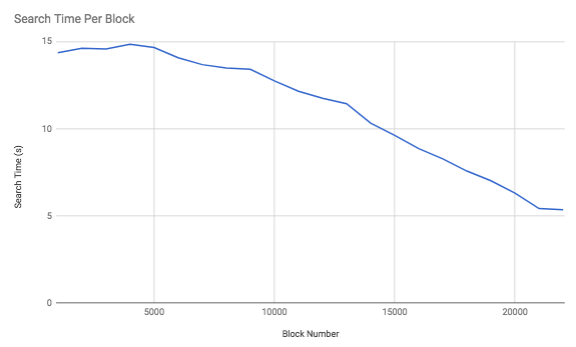
\includegraphics[width=0.9\columnwidth]{figures/draft-blocks.png}
 \caption{TODO
 \label{fig:opt}}
\end{figure}


\subsection*{Exp 5. Scaling}
\textbf{Sk. we exploit parallelism. This shows the stock dataset.}

\begin{table}[ht]
\centering
\label{my-label}
\begin{tabular}{|r|r|r|r|r|}
\hline
No Cores.   & No Cache & Cache Only & All Optimizations \\
\hline
1 & 4432.4 & 432.5 & 467.1 \\ \hline
2 & 2287.7 & 321.0 & 287.2 \\ \hline
4 & 1475.4 & 245.4 & 175.4 \\ \hline
8 & 806.5  & 206.2 & 106.7 \\ \hline
16 & 588.3  & 188.4 & 88.9  \\ \hline
32 & 378.1  & 162.1 & 78.4  \\ \hline
64 & 217.1  & 137.8 & 67.3    \\
\hline
\end{tabular}
\end{table}
